\chapter{Phase Retrieval}
%As discussed in the previous chapter, the wavefront of the x-ray radiation is described by its amplitude and its phase. As there currently there exists no device capable of measuring the phase of x-ray radiation, in general there is no direct way of recovering the object from the measured diffraction pattern. 
The problem with missing phase information is well known and is called the phase problem. There are many ways to overcome it: for example in crystallography, homology modelling or the anomalous scattering of heavy atoms is exploited to retrieve phases \cite{Rossmann1972,Arndt1978}. In Fourier holography the interference between two wave fields is used to obtain the phases \cite{McNulty1992, Eisebitt2004, Marchesini2008}. In ptychography the precisely known overlap and high redundancy between many exposures is used to solve the phase problem \cite{Rodenburg2007,Thibault2009}. In FXI the scattered field becomes oversampled, which means that, under certain conditions, phases can be retrieved from the intensity pattern itself. The next sections will describe oversampling in more detail, and explain how phases can be retrieved from an oversampled signal using iterative phase retrieval methods, and finally explain how phase retrieval can be validated. 

\section{Oversampling} 
In 1952 Sayre noticed, the Bragg peaks sample the molecular transform $\mathcal{F}(\rho)$ at the critical sampling rate ($\Pi_C$)\cite{Sayre1952a, Shannon1949a}\footnote{It was Bernal \cite{Bernal1938} that already noticed that the signal in between Bragg peaks could be sampled by hydrating and drying crystals.}. This means that if we know the phases in addition to the amplitudes at only the Bragg peaks, it is just enough to back-calculate the structure of the measured object. Single-particle imaging is free from the crystal lattice, and we obtain a continuous diffraction pattern. By choosing the detector distance appropriately such that individual pixels cover a small enough angle, we can sample the molecular transform more finely than the critical sampling rate. This sampling condition is called oversampling. Figure \ref{fig:sampling} illustrates both cases of sampling. 

\begin{figure}[h]
	\centering 
		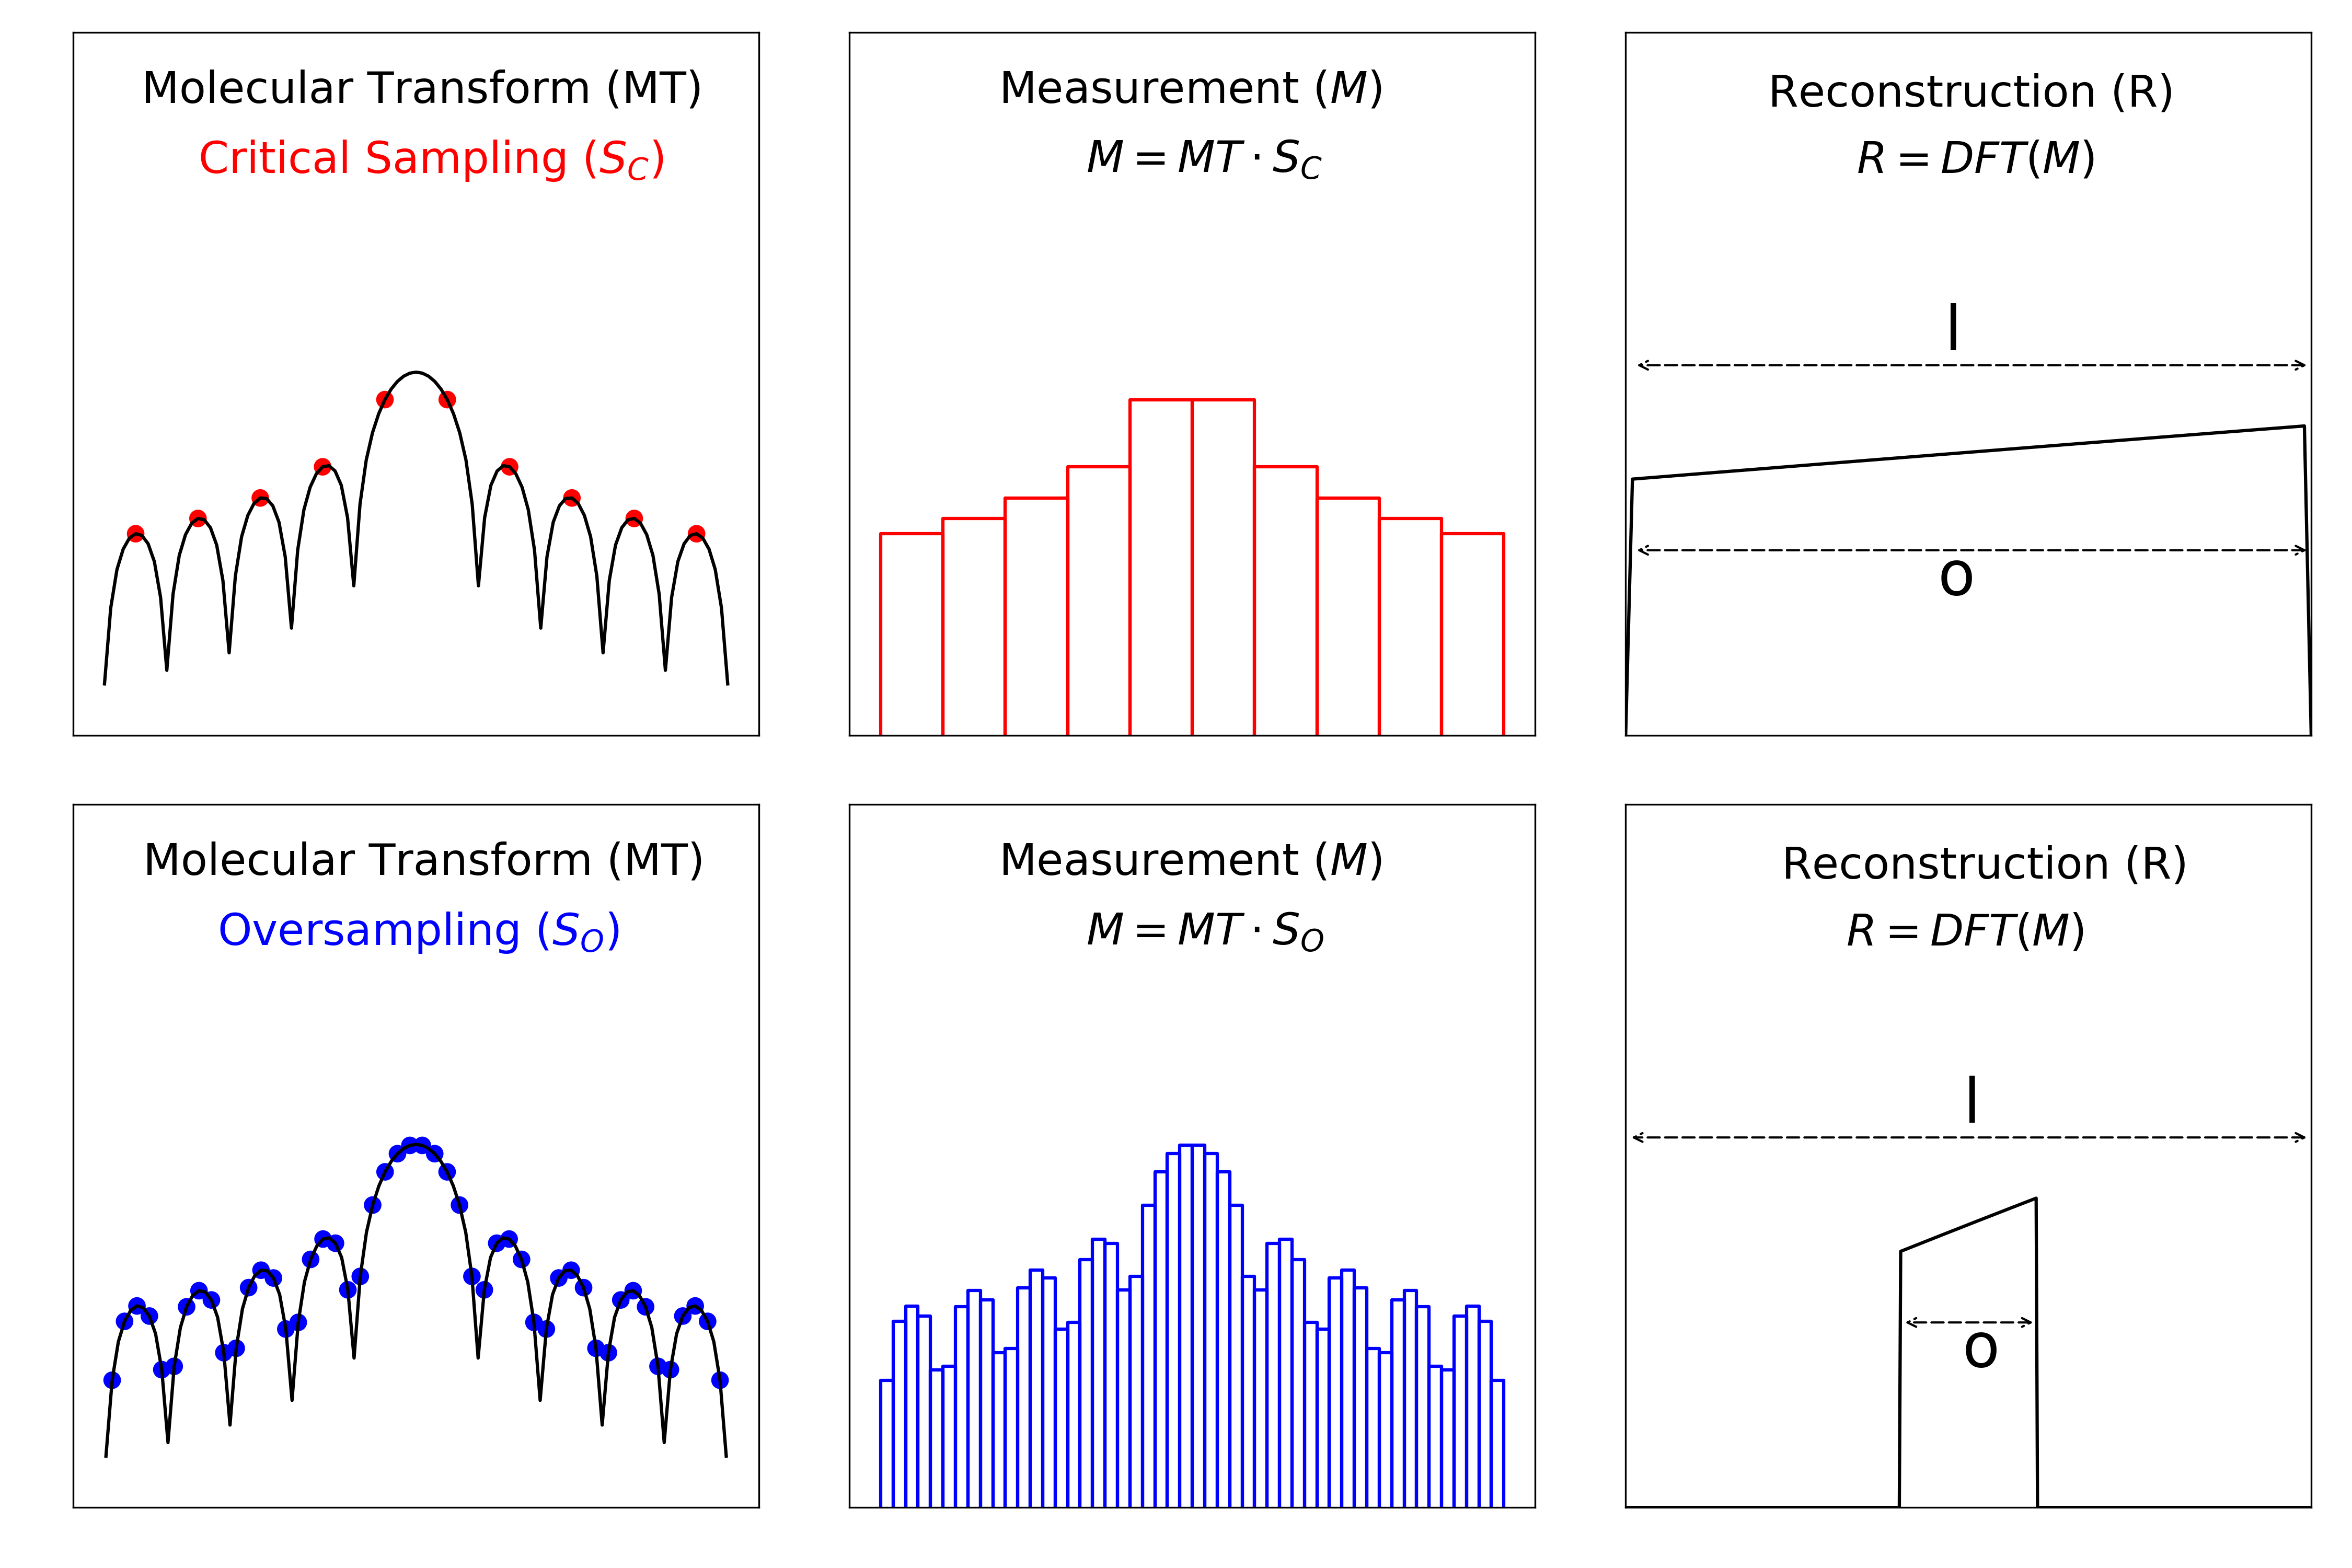
\includegraphics[width=120mm]{Chapter_06_Sampling.png}
	\caption{Illustration of critical sampling (top row) versus oversampling (bottom row). The right column shows two plots with an 1D signal in black. This signal corresponds to the molecular transform (MT) of our object. The MT is sampled at the critical sampling rate (top left), and an oversampling rate (bottom left). This is indicated by the red and the blue dots, respectively. The middle column shows what the measured signal, associated with the sampling rate, would look like. This bares resemblance to what is measured by a pnCCD. The right most column shows the DFT of both measurements. Important to note is that both DFTs show an similar reconstruction of the original object, but the size of the object compared to the field of view is different. The recovered object is exactly the size of the field of view when the molecular transform is sampled at the critical sampling rate. The size of the object is smaller than the field of view when the molecular transform is oversampled. Oversampling results in zero density around the recovered object.}
	\label{fig:sampling}
\end{figure}

If the oversampling is large enough the redundant information given by the extra sampling point is enough to retrieve the missing phases. The linear sampling rate $R_S$ is defined as the ratio between the actual sampling rate and the oversampling rate.

By choosing a detector setup such that the sampling rate is at least twice as high as the \cite{Bernal1938, Shannon1949a} the critical sampling rate we can use the additional intensity information to recover the missing phases, and thus reconstruct the object from the measured intensities alone. It has been proven that this method often has multiple solutions when applied to 1D data \cite{Walther1963}, however, for higher dimensions it does, in most cases, have a unique solution\cite{Bruck1979}. Oversampling is the basis of many phase retrieval techniques in single particle imaging, as well as some clever phasing techniques applied to Serial Femtosecond X-ray Crystallography (SFX) \cite{Ayyer2016,Chapman2011}.

\section{Iterative Phase retrieval}
In practice there are many ways to possibly retrieve the phase information from the diffraction pattern, but most common phase retrieval techniques are variations of convex optimization algorithms. This section introduces the general idea behind convex optimization, and explains three different algorithms in more detail.

As with many difficult problems, we start from the things that are known. Figure \ref{fig:sampling} shows that oversampling in Fourier space implies that there is an area  around the object with the size ($l-o$) for which we know the electron density $\rho(\vec{r})$ is zero. This knowledge can be used as a constraint on the possible phases. We know that a correct choice of phases would make the corresponding $\rho(r)$ zero in this area. The area that can contain the sample density  and therefore contains nonzero electron density is called the support $M(\vec{r})$. This constraint is called the real-space constraint. Furthermore, we know that the recovered Fourier amplitudes should agree with the measured intensities. This is called the Fourier-space constraint. 

In 1978 Fienup \cite{Fienup1978} introduced an algorithm called Error Reduction (ER) to solve the phase problem. It was inspired by an earlier algorithm by Gerchberg and Saxton \cite{GerchbergSaxton1972}, but applied to the phase problem. ER is an iterative approach that tries to find a solution that minimizes the disagreement with both the real-space constraint and the Fourier constraint. In words it can be described as follows:\\
\begin{enumerate}
\item Assign random phases to each pixel in Fourier space.
\item Inverse Fourier transform to get the corresponding real space.
\item Set all electron density outside the support to zero, keep the electron density inside the support unchanged.
\item Fourier transform the new density to get the corresponding Fourier space.
\item Make the recovered amplitudes match the measured intensities. Keep the phases unchanged.
\item Go back to step 2.\\
\end{enumerate}


ER is sometimes able to find the correct solution, but because the problem is not convex it often gets stuck in local minima and does not find the global solution.

In 1984 Levi and Stark realized that the two constraints described above can be interpreted as projections in a multidimensional Hilbert space \cite{Levi1984}. Step 3 will from now on be called the real-space projection $P_r$. The sequence of step 4,5 and 2 will be called the Fourier Projection $P_f$.  In ER $P_r$ and $P_f$ can be defined as follows:
\begin{align}\label{eq:ER}
P_r \rho\left(\vec{r}\right) =& \begin{cases} \rho\left(\vec{r}\right) \quad &\mathrm{if}\,\,
    \vec{r} \in M\\0 \quad & \mathrm{if}\,\, \vec{r} \not\in M \end{cases}\\
P_f \rho(\vec{r}) =& \mathcal{F}^{-1}\left( \frac{\sqrt{I}}{|\mathcal{F}(\rho(\vec{r}))|}\mathcal{F}(\rho(\vec{r})) \right)
\end{align}

The largest difference between the two projections is that the support constraint is convex, while the Fourier constraint is not. An iteration in ER can now been seen as a real-space projection followed by a Fourier projection. A common and flexible way to express one iteration of the algorithm is by the following equation:
\begin{equation}\label{eq:fom}
\rho_{n+1}\left(\vec{r}\right) = \begin{cases} P_f\rho_{n}\left(\vec{r}\right) \quad &\mathrm{if}\,\,
    \vec{r} \in M\\0 \quad & \mathrm{if}\,\, \vec{r} \not\in M \end{cases}
\end{equation}

Two error metrics can be constructed by measuring the change imposed by the respective projection:	the Fourier error, $E_f$, and the real space error,$E_r$. Intuitively, $E_r$ measures how much of the electron density outside the support. $E_f$ gives the difference between the measured and the recovered amplitudes and the square root of the intensities. Mathematically $E_f$ and $E_r$ are defined as:

\begin{equation}
E_r = \left|P_r\rho(\vec{r}) - \rho(\vec{r})\right| = \left(\sum_i\rho_i^2\right)^{\frac{1}{2}}
\end{equation}

\begin{equation}
E_f = \left|P_f\rho(\vec{r}) - \rho(\vec{r})\right| = \left(\sum_{i}\left(\frac{\sqrt{I_i}}{|F(S_i)|}- F(S_i)\right)\right)^{\frac{1}{2}}
\end{equation}
  
\subsection{The Hybrid Input Output algorithm (HIO)}
In 1982 Fienup introduced an algorithm that can escape from local minima, the so-called the Hybrid Input Output algorithm (HIO) \cite{Fienup1982}. To achieve this HIO makes use of a relaxation parameter called $\beta$. An iteration of HIO can be described as follows, using the same syntax as in equation \ref{eq:fom}:
\begin{align}
\rho_{n+1}\left(\vec{r}\right) = \begin{cases} P_f \rho_{n}\left(\vec{r}\right) \quad &\mathrm{if}\,\,
    \vec{r} \in M\\\rho_n(\vec{r}) -\beta P_f \rho_n(\vec{r}) \quad & \mathrm{if}\,\, \vec{r} \not\in M \end{cases}
\end{align}

I consider the $\beta$ parameter in a similar way as the temperature in simulated annealing. If $\beta$ is large the algorithm can escape deeper local minima. Unfortunately this also means that the global minima might be escape as well. If $\beta$ is small HIO will miss fewer minima, but will have greater difficulty escaping from them. As long as a minimum is not perfect ($E_r$ and $E_f$ are both nonzero), HIO will, given enough time, eventually be able to escape.

\subsection{The Relaxed Averaged Alternating Reflections algorithm (RAAR)}
Another algorithm that is often used in the work described in this thesis is the Relaxed Averaged Alternating Reflection algorithm (RAAR). RAAR does not escape all minima but it can escape shallower ones. For high-quality data RAAR seems to find the solution quicker and more reliably than HIO. An iteration of RAAR can be described as follows:
\begin{align}
\rho_{n+1}\left(\vec{r}\right) = \begin{cases} P_f \rho_{n}\left(\vec{r}\right) \quad & \mathrm{if} \,\,
    \vec{r} \in M\,\mathrm{and}\,\rho_n(\vec{r}) \geq -(1+\beta)P_f\rho_n(\vec{r}) \\\
    \beta\,\rho_n(\vec{r}) -(1-2\beta) P_f \rho_n(\vec{r}) \quad & \mathrm{if}\,\, \mathrm{otherwise} \end{cases}
\end{align}

As both RAAR and HIO do not guarantee to end up in the bottom of a minimum, concluding phase recovery with a number of iteration of ER will ensure that the final solution is close to a minimum. This can improve the overall quality of the reconstruction, as shown in \textbf{Paper I}.

\subsection{Other algorithms}
There exist many other phase recovery algorithms (See \cite{Marchesini2007a}). A software package called Hawk \cite{Maia2010} allows users to select and test different algorithms. Hawk is especially powerful as it is fast and gives direct graphical feedback about the reconstruction process. The latter can for example be very useful in determining the correct support size. 

\section{Shrinkwrap}
While HIO and RAAR perform well when the support is well known and follows the shape of the actual object tightly. In practise this information is often not available and phase retrieval can become practically impossible if the support is too large. In 2003 Marchesini developed an algorithm called Shrinkwrap \cite{Marchesini2003} that does not require an \textit{a priori} known support as input, but instead tries to deduce the shape of the support during the reconstruction. After each $n$ iterations the support is updated by applying a Gaussian blur to the real space image and selecting the pixels that have a value above a certain threshold. The general idea is that even with a somwhat inaccurate support, some features will be recovered well, and by using these features the support will become a bit better, which in turn allows for more feautres to be recovered. The algorithm has been very successful for experimental data \cite{Seibert2011}.

\section{Validation}

\subsection{Errors}
The most basic method to assess the difference in quality between two reconstructions is by comparing the respective errors. The reconstruction with lower errors is generally believed to be a more correct reconstruction. This method does however not teach us anything about the biological validity of a reconstruction and is most often only used to exclude clearly failed reconstructions that will have errors that clearly deviate from the successful ones.
 
\subsection{PRTF}
A standard tool to assess the quality of a reconstruction is the phase retrieval transfer function (PRTF). This function measures the variation within a set of independent reconstructions from the same data but different random starting phases. The PRTF can then be used to quantify the resolution of a reconstruction. The underlying assumption is that any feature that is reproducibly recovered is likely to be a true feature, but non-reproducible features are artifacts caused by the particular starting phases. The variation between reconstructions is calculated for each pixel $i$ in Fourier space by adding together all the recovered amplitudes for that pixel and dividing the total vector by square root of the measured intensity for that pixel $v_i = |\frac{\sum A_i}{\sqrt{I_i}}|$. If the value of $v_i$ is close to unity, all reconstructions recovered a similar amplitude for that pixel. The closer $v_i$ is to zero the more difference is there between the individual reconstructions. The most common way to present the PRTF is to plot the radial average of $v_i$. This plot can be interpreted as a measure of reconstruction quality as a function of resolution. A common practice in the field is to quantify the resolution of a reconstruction by the first time the 1D PRTF drops below the ,somewhat arbitrary, threshold 1 / $e$ (See \cite{Seibert2011}). The corresponding resolution is given by the inverse of the distance to the origin. The real-space solution is presented as the average of all reconstructions that are included in the PRTF. In this image, non-reproducible features will be averaged out and only the reproducible features will be left.
 
\subsection{Missing Mode Analysis}
As described earlier, diffraction patterns often lack data in certain regions. Even in the best case the central region will be missing because the direct beam would otherwise damage the detector. The other main sources of missing data gaps between detector tiles and saturation. 

Reconstruction algorithms deal with this missing data by recovering the amplitude as well as the phase for the pixels in these regions. In many cases the missing data does not affect the stability of phase recovery, this is however not true general. To understand when this happens we have to note that the Fourier constraint does not constrain the amplitudes in the missing data area, and the real-space constraint does not limit the electron density inside the support. If there exists an object that can fit inside the support and has a Fourier transform that is zero outside the missing data region, this object would be completely unconstrained. Such an object could be arbitrarily added to the solution without changing how well the solution forfill the constraints and this would mean that there is not unique solution.

In practice completely unconstrained objects do not exist. Objects that fit inside the support and only slightly contribute outside of the missing data region can however exist. We call such objects weakly constrained. In the design of an experiment, or when deciding whether or not to phase an object it is important to predict whether weakly constrained objects exist for that particular data. This analysis is called missing mode analysis and the weakly constrained objects are usually called modes.

The DFT can be represented in matrix form, where each column represents a pixel in real space and each row represents a pixel in Fourier space. Real space and Fourier space will then each be a vector and the transform itself will be a multiplication with the DFT matrix. The elements in the input and output vectors can be rearranged arbitrarily as long as the corresponding rows and columns of the DFT matrix is rearranged in the same way. Here we have rearranged the pixels so that the unconstrained pixels, i.e. the pixels that are in the support or masked out, come first.


\begin{equation}\label{equ:F_split}
  \mathcal{F} = 
  \left(\begin{array}{l|lll}
    \mathcal{F}_{SM} & &\mathcal{F}_{\bar{S}M}& \\\hline
    &&&\\
    \mathcal{F}_{S\bar{M}} & & \mathcal{F}_{\bar{S}\bar{M}} &\\
    &&&
  \end{array}\right)
\end{equation}

In the matrix above the bar indicates the inverse of the support , $S$, and mask, $M$, respectively. We are only looking for objects that only have values in $S$ and minimize the contribution outside the mask. This means that we need to minimize $|\mathcal{F}_{S\bar{M}}\rho|$. A common method to find such objects is singular value decomposition \cite{Eckart1936}. This method decomposes $|\mathcal{F}_{S\bar{M}}\rho|$ into a diagonal matrix $\Sigma$, and two unitary matrices $U$ and $V$. The values in $\Sigma$ are called singular values. The smallest singular values correspond to the most weakly constraint objects, or weakly constrained modes.

\subsection{Hierarchical Clustering}
As the reconstruction process might end up in different solutions, we typically use the Fourier and real-space error to select what particles to keep for the PRTF. The assumption here is that failed reconstructions have higher error scores that the successful ones. 

I conducted a study to test whether this practice actually selects
In \textbf{Paper I} we used the  UPGMA (Unweighted Pair Group Method with Arithmetic Mean) hierarchical clustering method \cite{Sokal1958} to determine the number of structurally different solutions present in the set of reconstructions. The workflow of this method is illustrated in Figure \ref{fig:UPGMA}.

\begin{figure}[h]
	\centering 
		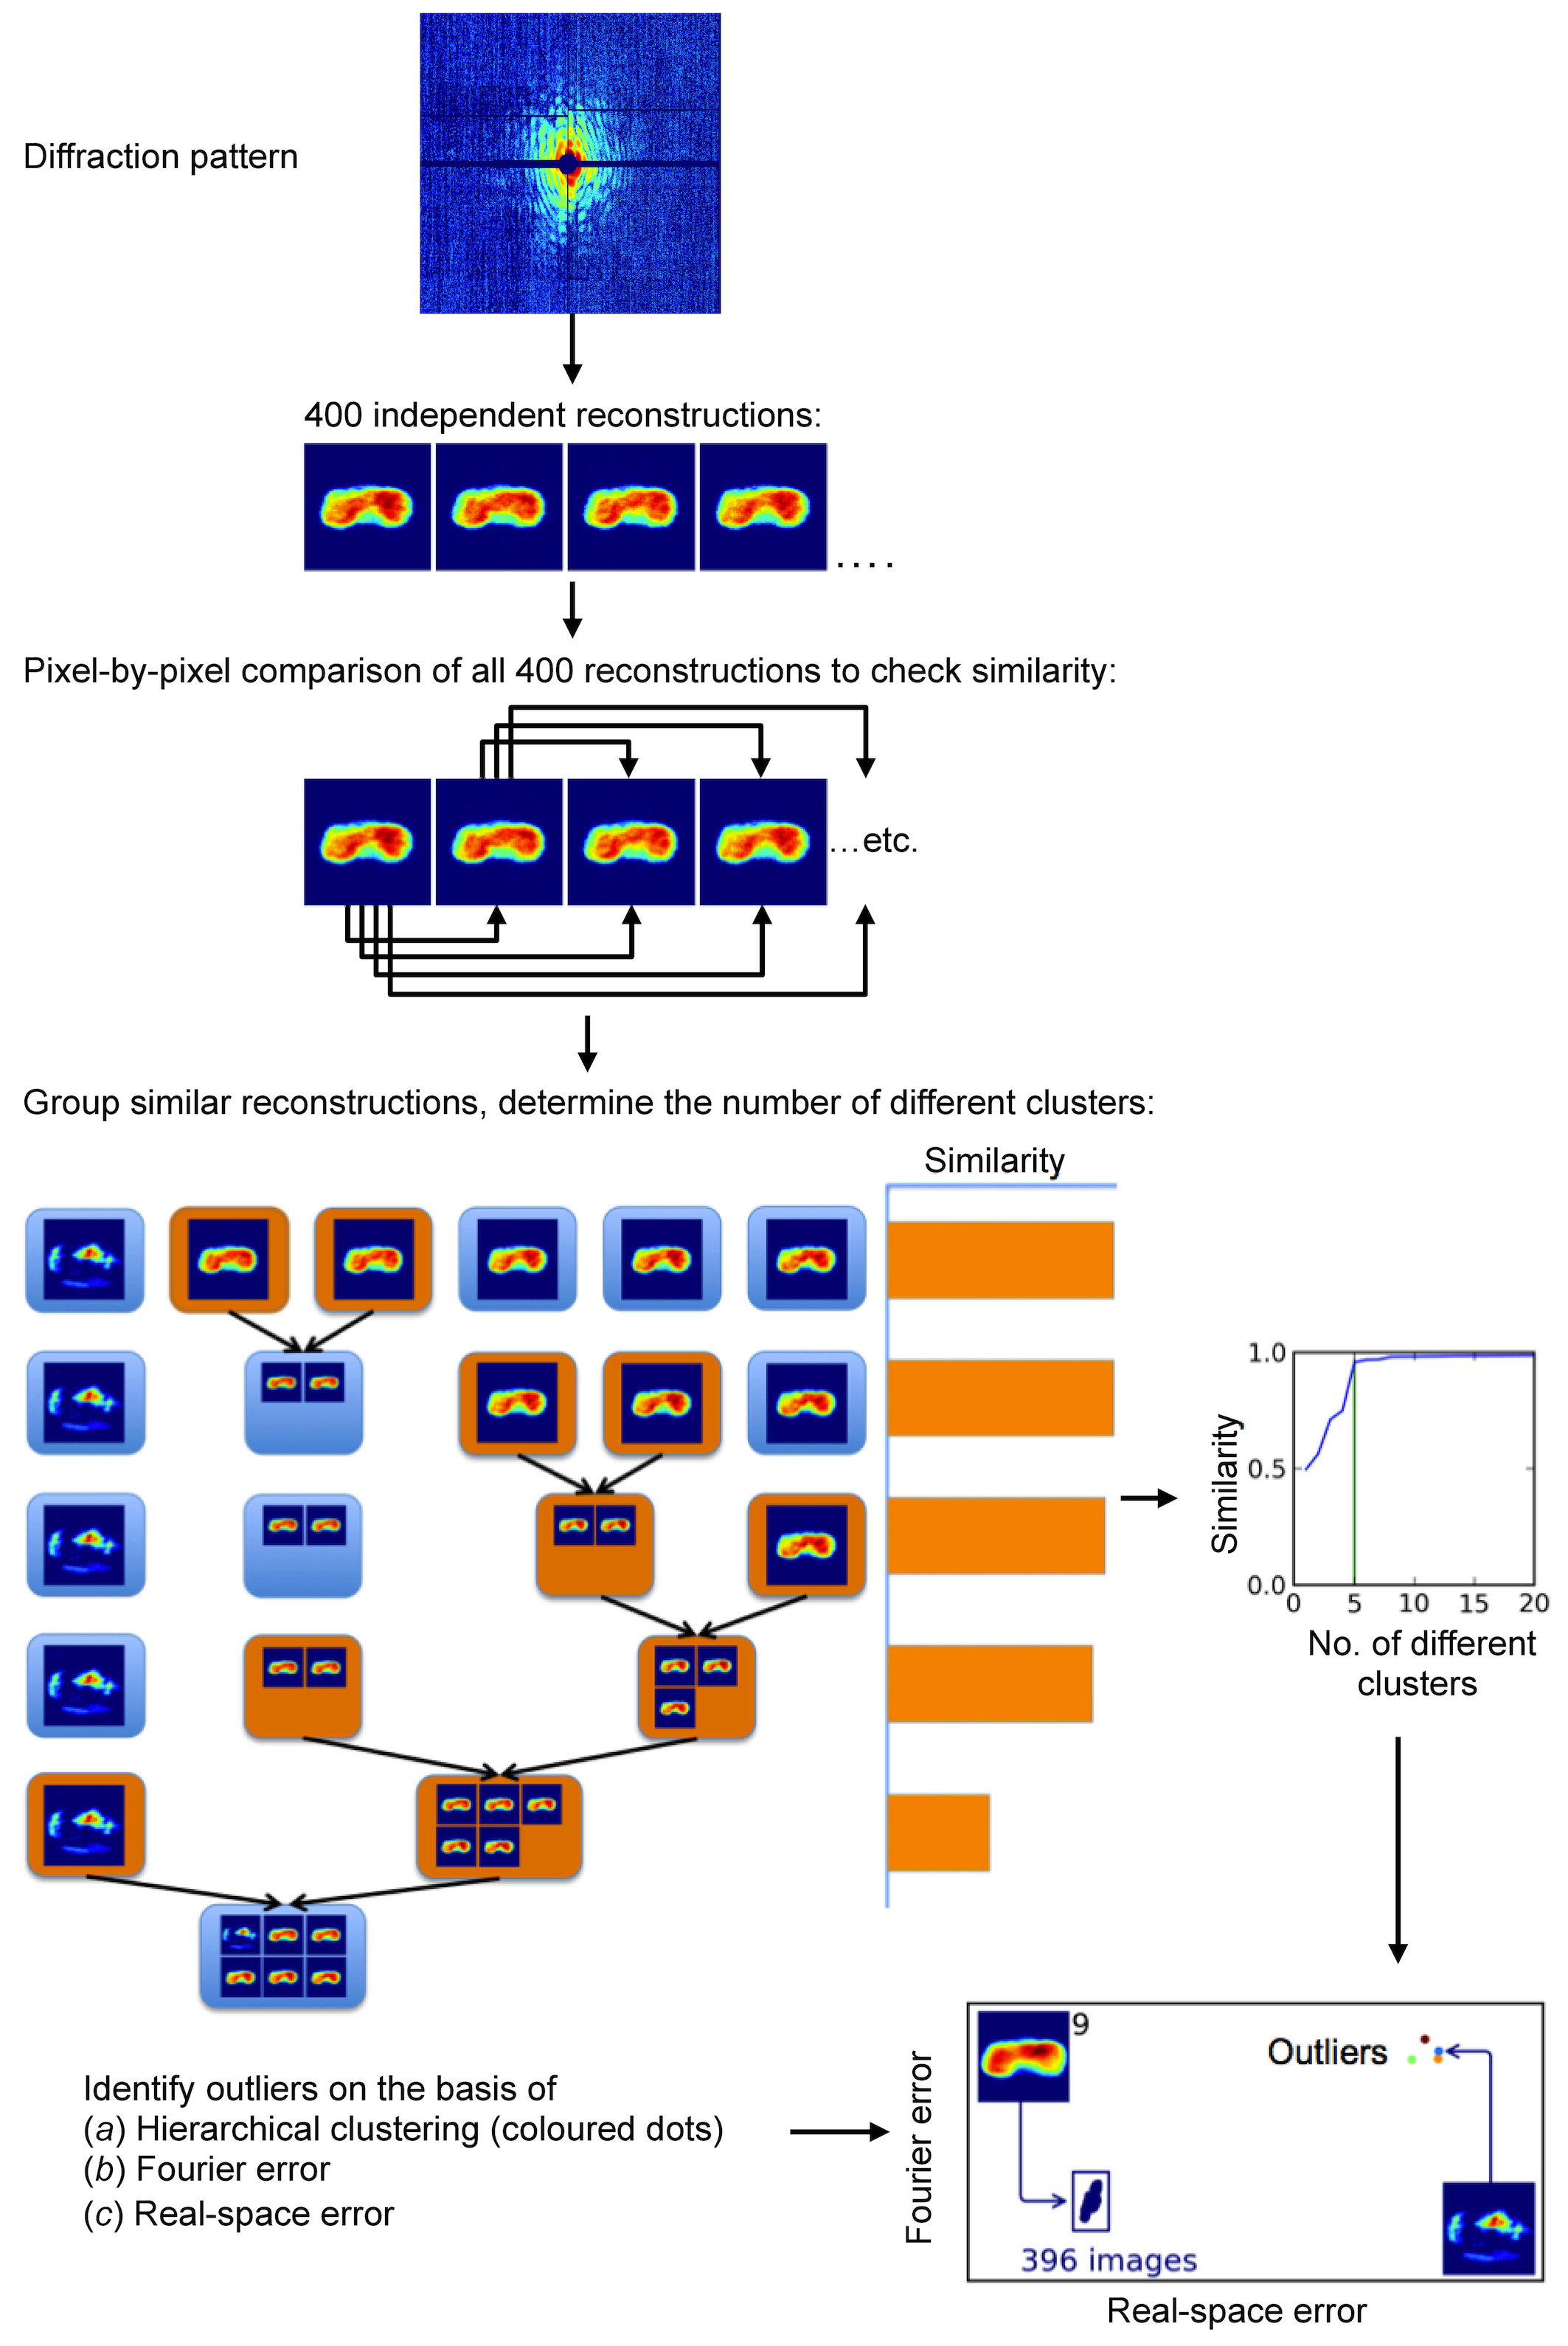
\includegraphics[width=100mm]{Chapter_06_UPGMAClustering.jpg}
	\caption{Flow chart of the UPGMA Clustering algorithm. In the first step of the algorithm, n independent reconstructions (400 in this example) are compared pairwise, pixel-to-pixel to check similarity. Each comparison results in a so called comparison score. The second step is the actual clustering step in which the number of different clusters present in the set of reconstruction is determined. Initially each reconstruction belongs to its own cluster. In each consecutive merging step the two most similar clusters are merged into one cluster. This repeats itself until one cluster remains. Each merge can be given a similarity score using the comparison	scores from step 1. By plotting the similarity scores against the number of clusters, the number of clusters can be determined. We choose the number of cluster by cheking where this plot makes a kink. This is indicated by the green line in the top graph on the right. The bottom plot shows the Fourier-error and the Real-space error associated to each reconstruction, color-coded on the basis of which cluster they belong to. Here we note that there are four outliers and one main cluster. The outliers are clearly failed reconstructions.}
	\label{fig:UPGMA}
\end{figure}

In the first step of this method each reconstruction is compared pairwise to every other reconstruction, pixel-to-pixel. The comparison score associated with each comparison is the normalized scalar product between the pair of reconstructions, after translating them to their optimal fit. 

In the second step of the method similar reconstructions are grouped in clusters. Initially each reconstruction belongs to its own cluster. In every consecutive step the two most similar clusters are merged into one cluster, until in the end only one big cluster remains. For each merge we calculate a similarity score, which is the average comparison score for all reconstruction in the merged cluster. We plot the similarity score of each cluster merge as a function of the number of clusters. The agglomeration step where the plot makes a "kink" is chosen as the number of different clusters that are present in the set of reconstructions. This is a standard way to estimate the number of clusters present in the set of reconstructions. This capability is an advantage of the  clustering algorithm. 

In a 2D plot of $E_f$ vs. $E_r$, color-coded by cluster, it is possible to see whether or not there is a correlation of reconstruction similarity and error score.  In the case that several large clusters remain after applying a real-space error and Fourier-error threshold the clusters have to be examined carefully. If the remaining clusters correlate with the errors we suggest to keep only the cluster with the lowest error. If no correlation is present between score and cluster it is advised to keep all clusters for further evaluation, because otherwise there is a possibility of selecting on similarity, which would negate the validation power of the PRTF.

 
\section{Simulated Phase Contrast Methods}
Once the phase of the diffraction pattern is retrieved, one has complete knowledge of the information encoded in the  wave-field. This total knowledge is powerful, because it allows the emulation of the action of any imaging system for which an associated mathematical transform can be written, regardless of its experimentally feasibility.
For example, differential interference contrast imaging, otherwise known as Nomarski imaging, is experimentally a well-established technique to visualize the changes in phase \cite{Nomarski1955}. This change can have biological meaning, for example the density inside certain organelles can be higher than the average density in cells. Normarski imaging will give a more pronounced image of the borders of the organelle. For an example see ref \cite{Barty1998}. 

Nomarkski imaging in its simplest form takes a scattered wave-field, say $\psi(x,y,z = 0)$, and then interferes this wave-field with a copy of itself that has been given both a slight transverse displacement ($\Delta x$, $\Delta y$) and a phase shift $\phi_0$. Thus the intensity of the resulting wave-field $F_N$ is \cite{Paganin2004}:
$|\psi(x,y,z=0)+ e^{(i\phi_0)} \psi(x - \Delta x,y - \Delta y,z=0) |^2$, from which one can show (using the Fourier shift theorem) that the transfer function becomes:
\begin{equation}
\begin{aligned}
\begin{split}
T_{DIC}(q_x, q_y, \tau) = 1 + e^{(i(\phi_0 - q_x \Delta x - q_y \Delta y))},\\
\tau = (\phi_0, \Delta x, \Delta y)
\end{split}
\end{aligned}
\end{equation}

In the case of a reconstructed image $\rho(\vec{r})$, the Normarski variant $N$ will look like:
\begin{equation}
N = \mathcal{F}^{-1} T_{DIC} \mathcal{F}(\rho(\vec{r}))
\end{equation}
We have created simulated Nomarski images of the reconstructed cell images shown in the results part.



